\section*{Abstract}
A sound understanding of plant growth is critical to maintaining future crop productivity under ongoing climate change. Remotely sensed time series of crop functional traits from optical satellite imagery are an invaluable tool for deriving appropriate management practices that facilitate risk mitigation and increase the resilience of agroecosystems. However, the availability of imagery is limited by atmospheric disturbances that cause large temporal gaps and noise in the trait time series. 
Therefore, time series reconstruction methods are required for accurate crop growth modelling. Physiological priors, such as the fact that plant growth is mainly controlled by a few environmental covariates, among which air temperature plays a prominent role, represent a promising approach to improve the representation of crop growth. Here, a novel approach is proposed that combines Sentinel-2 Green Leaf Area Index (GLAI) observations with three dose response curve approaches describing the a priori physiological relationship between growth and temperature in winter wheat. A probabilistic ensemble Kalman filtering data assimilation scheme allows the combination of high temporal resolution air temperature data and satellite imagery, which also allows quantification of uncertainties. 
The proposed approach requires a smaller number of satellite observations compared to conventional remote sensing time series algorithms, making it suitable for agricultural areas with high cloud cover, and is considerably less complex than a mechanistic crop growth model. Validation was carried out using in-situ data collected on winter wheat plots in Switzerland in two consecutive years. The validation results suggest that the proposed assimilation of Sentinel-2 GLAI and temperature-response-based growth rates allows the reconstruction of physiologically meaningful GLAI time series. In particular, the systematic underestimation of high in-situ GLAI values (> 5 $m^2$ $m^{-2}$) often prevalent in purely remote sensing driven GLAI time series reconstruction was reduced. Thus, the proposed approach is advantageous compared to state-of-the-art remote sensing approach based on wide-spread logistic functions by means of physiological plausibility, fitting requirements and representation of high in-situ GLAI values. This has great potential to increase the reliability of remotely sensed crop productivity assessment.

\section{Introduction}
\label{sec:introduction}
The majority of daily calorie intake is provided by a few arable crops, including wheat. Ongoing climate change poses a major challenge to the ability of such crops to produce resilient yields \citep{asseng_rising_2015}. This calls for suited management practices to mitigate risks and increase the resilience of agroecosystem. Consequently, a sound understanding of plant growth is urgently needed to identify and minimise crop risks \citep{tilman_global_2011}. Plant growth dynamics within different phenological phases can be of great interest to identify stressors \citep{reynolds_physiological_2016}. An important phase with respect to the yield potential of winter wheat (\textsl{Triticum aestivum}) is the stem elongation phase (i.e., begin of stem elongation until begin of flowering), which will be the focus of this study \citep{kronenberg_monitoring_2017, miralles_duration_2000}.

Using optical satellite remote sensing, plant growth can be recorded on large spatial scales with relatively high temporal resolution. Remotely sensed time series of functional crop traits such as \gls{GLAI} -- defined as the photosynthetically active leaf area per unit ground area ~\citep{maddonni_leaf_1996} -- are therefore widely used to estimate vegetation productivity ~\citep{kooistra_reviews_2023}. For time series reconstruction, mainly statistical models are used, which fit a function to a set of satellite observations. Over the past decades, a variety of these statistical reconstruction models have been proposed  \citep{zeng_review_2020, kooistra_reviews_2023}. These models range from simple linear interpolation to models that already incorporate prior knowledge about vegetation development, such as \gls{DL}~\citep{beck_improved_2006}. \gls{DL} take advantage of the fact that most crop traits follow a bell curve with an ascending branch for the generative phase and a descending branch for the senescent phase. \gls{DL} are therefore a clear advancement compared to time series reconstruction methods such as the Savitzky-Golay filter \citep{savitzky_smoothing_1964}, the Whittaker smoother \citep{eilers_perfect_2003}, or Gaussian processes regression \citep{belda_optimizing_2020, pipia_green_2021} that lack a explicit formulation of basic principles of crop growth and development. \gls{DL} can be used to plausibilize the estimation of functional crop traits, i.e., to check whether temporal trajectories are consistent with prior knowledge~\citep{koetz_use_2005}. Strictly speaking, this reconstruction is a modeling of crop growth.

Still, even such advanced models depend on the availability of a sufficiently high number of satellite observations. The number of observations in optical remote sensing, however, can be reduced significantly by unfavorable atmospheric conditions such as clouds. In mid-latitude environments, which represent a major part of the world's wheat production area, the percentage of cloudy optical satellite images can be higher than  60\%~\citep{sudmanns_assessing_2020}. This leads to larger temporal gaps in the data which constrain time reconstruction accuracy~\citep{zhou_reconstruction_2015}. Moreover, undetected clouds and shadows, i.e., noise, can deteriorate the quality of time series reconstruction~\citep{zhou_performance_2016}. This is significant as the reconstruction methods approach crop growth modeling mainly from a statistical perspective, i.e., they make strong assumptions about the distribution and power of signal and noise. Moreover, the model parameters of statistical methods such as the aforementioned Whittaker smoother or Savitzky-Golay filter have often no intrinsic biological or physical meaning. Thus, the physiological plausibility of the reconstructed time series is not guaranteed resulting in a potentially misleading representation of crop growth. Nevertheless, the acceptance of these models in the remote sensing community is high~\citep{kooistra_reviews_2023} as the models are usually fast and easy to use.

A more advanced perspective on crop growth and development is provided by mechanistic crop models that address the underlying physiological processes~\citep{delecolle_remote_1992, jamieson_sirius_1998,keating_overview_2003}. Mechanistic, or process based, models are explicit formulations of physical and biological processes, with physical and biological meaning assigned to all parameters of the model \citep{cox_towards_2006}. However, these models require extensive calibration efforts and information about boundary conditions such as soil properties which are often not available. To address this issue, the assimilation of remotely sensed functional traits has been proposed~\citep{pellenq_methodology_2004} and shown to improve vegetation productivity estimation~\citep{huang_assimilation_2019, waldner_high_2019}. Still, the complexity of mechanistic models and lack of calibration data limit their use in agricultural remote sensing~\citep{weiss_remote_2020} although more simpler models such as the \gls{SAFYE} have been proposed \citep{ma_wheat_2022}.

From a purely physiological perspective, temperature is one of the most important and yet easy to measure covariates controlling plant growth~\citep{porter_temperatures_1999, asseng_climate_2019}. A simple and widely used example in this regard is the concept of \gls{GDD}~\citep{mcmaster_growing_1997}. \gls{GDD} describe the change of a trait value, i.e., growth, as the accumulation of temperature sums. This, however, partly neglects the effect that any chemical and, hence, biological process takes place within a specific temperature range and that reaction (growth) rates are a function of temperature. In detail, there is a minimum or base temperature $T_{base}$ below which no growth occurs as well as a maximum temperature $T_{max}$ above which growth comes to a halt. Between $T_{base}$ and $T_{max}$ there is an optimal temperature, $T_{opt}$, at which the growth rate reaches its maximum~\citep{porter_temperatures_1999}.

Various \gls{DRC}s have been proposed to model growth as a function of temperature \citep{wang_uncertainty_2017}. The range of functions varies from the above \gls{GDD}s to the use of more complex functions such as asymptotic curves \citep{roth_phenomics_2022}, the curve proposed by \cite{wang_simulation_1998} or the Arrhenius-shaped curve proposed in \cite{parent_temperature_2012}. The parameters of the \gls{DRC}s have -- like mechanistic crop models -- a biological meaning, but require only a few parameters, which arguably makes them easy to use. ~\citet{roth_phenomics_2022} have shown that crop growth rates under field conditions can be accurately reconstructed from \gls{DRC}s. The authors have also shown that \gls{DRC}s based on hourly air temperature data allow interpolation of coarser resolution (every three to four days) trait observations. However, to the best of our knowledge, a \gls{DRC}-based time series reconstruction approach has not been used to interpolate between satellite-derived crop trait observations.

Our primary objective is therefore to use a priori physiological knowledge of the dependence of plant growth on air temperature encoded in \gls{DRC}s to improve the reconstruction of \gls{GLAI} time series from a set of satellite observations. We hypothesise that the use of physiologically informed \gls{DRC}s and high spatial resolution trait observations will provide an accurate, physiologically consistent representation of crop growth. We therefore assume \gls{DRC}s to outperform statistical time series reconstruction methods that lack an explicit linkage to biology.

Based on our objective, we formulate three research questions:

\begin{itemize}
    \item First, can \gls{DRC} crop growth rates be used to reconstruct continuous, physiologically plausible crop trait time series from a set of satellite observations?
    \item Second, does the proposed approach outperform a time series reconstruction based on remote sensing data alone in terms of accuracy and reliability?
    \item Third, what temporal resolution of temperature data is required - hourly or daily?

\end{itemize}

To address these questions, we focus on \gls{GLAI} derived from the \gls{S2} satellite constellation at a study region in Switzerland, which acts as a blue-print for intensively farmed agricultural landscapes in temperate climate zones.

We start with a description of the in-situ \gls{GLAI} data used to calibrate and validate our proposed methodology (Section \ref{sec:drc_study-area-data}). We then describe the fitting of the \gls{DRC}s to encode a-priori physiological knowledge. We continue with the \gls{GLAI} retrieval from \gls{S2} to introduce spatial detail and large area coverage, and the proposed probabilistic reconstruction scheme in Section \ref{sec:drc_methods} alongside a baseline method based on \gls{S2} \gls{GLAI} observations, only.

\section{Data}
\label{sec:drc_study-area-data}
\subsection{Data}
\subsubsection{Calibration Data}
\label{subsec:calibration-data}

Three sites in Switzerland (CH Bramenwies), western (Rur catchment, DE-Rur) and south-eastern Germany (Munich-North-Isar, DE-MNI) were used for calibration, i.e., for establishing the physiological a-priori knowledge. The data cover several winter wheat growing seasons. The sites represent winter wheat field parcels operated by farmers according to local agricultural management practice (see Table~\ref{tab:Calibration_data_overview} for an overview).

At all sites, \gls{GLAI} measurements (section \ref{subsubsec:glai-processing}) and phenology (section \ref{subsubsec:phenology-processing}) ratings were carried out, which were linked to hourly air temperature from nearby weather stations. The \gls{GLAI} measurements were chosen to represent the generative phase of the growing season, within which the \gls{GLAI} should increase over time, i.e., the beginning of stem elongation to heading. In total the calibration data set contains 890 data points with the corresponding temperature history (Table~\ref{tab:Calibration_data_overview}). The dataset contains a total of 11 environments (year $\times$ location), providing a representative data set for model calibration in temperate environments of central Europe. Further details about the sites are provided in the following paragraphs.

\begin{table}[H]
\caption{Calibration data with locations, years, the corresponding amount of \gls{GLAI} measurements, and reference of the dataset. Latitude and longitude are provided in geographic coordinates (WGS-84).}
\label{tab:Calibration_data_overview}

\centering
\begin{tabular}{llllll}
Location      & Years                                                                        & \begin{tabular}[c]{@{}l@{}}\gls{GLAI}\\measurements\end{tabular}  & Lat. & Lon. & Reference \\ \hline
CH Bramenwies & 2022  & 840   & 47.45 & 8.69     & ~\cite{wildhaber_assessing_2023}          \\
DE MNI        & \begin{tabular}[c]{@{}l@{}}2017, 2018,\\ 2020, 2021,\\ 2022\end{tabular} & 24   & 48.29 & 11.71 &  \begin{tabular}[c]{@{}l@{}}~\cite{danner_retrieval_2017},\\~\cite{danner_fitted_2019},\\~\cite{wocher_physically-based_2018}\end{tabular}         \\
DE Rur        & \begin{tabular}[c]{@{}l@{}}2008, 2009,\\ 2010, 2013,\\ 2015\end{tabular} & 26   &  50.87 & 6.44 & \cite{reichenau_comprehensive_2020}       \\
\hline
\end{tabular}
\end{table}

\paragraph{CH Bramenwies}
At the Bramenwies site in northern Switzerland ($47.45^\circ$ N, $8.69^\circ$ E, 550 m above sea level), 840 \gls{GLAI} were measured within a single winter wheat field parcel (2.04 ha) at 29 predefined sampling points during the growing season of 2022. The area receives a total annual precipitation of 1200 mm and has an annual air temperature of 10 °C (reference period 2011 to 2022). The soil of the moderately sloping parcel is loamy (clay content 20 to 30\%) and slightly alkaline (pH between 7.2 and 7.8) with moderate humus content (3.0 to 3.6\%). The parcel was managed according to Swiss standards for conventional agriculture with three applications of mineral fertiliser in April and May 2022 \citep{wildhaber_assessing_2023}. Meteorological data were available from a weather station operated by the Agrometeorological Network of the Institute for Excellence in Agricultural Research, Agroscope.

\paragraph{DE MNI}
24 \gls{GLAI} measurements in winter wheat from five years between 2017 and 2022 were available at the MNI site ($48.29^\circ$ N, $11.71^\circ$ E, 440 m above sea level) close to the river Isar ($\le$ 10 km) north of the city of Munich. Measurements were taken between the beginning of April and July each year. The average annual air temperature is about 8.9 degrees Celsius with an annual precipitation of 757 mm (reference period 1991 to 2020). The dominant soil types in the mostly flat area are gleysols and pararendzina of alluvial origin. The parcels were managed according to conventional agricultural practices following German standards \citep{danner_retrieval_2017, danner_fitted_2019, wocher_physically-based_2018}. Weather data was obtained from a station operated by the German Meteorological Service at Munich Airport.

\paragraph{DE Rur}
At the Rur catchment in northwestern Germany, 26 \gls{GLAI} measurements were made in five years between 2008 and 2015 ($50.87^\circ$ N, $6.44^\circ$ E, 100 m above sea level) in a fertile loess plain characterised by luvisols and anthrosols \citep{reichenau_comprehensive_2020}. From the original dataset of \cite{reichenau_comprehensive_2020} we took \gls{GLAI} observations in winter wheat from the sites Merzenhausen, Selhausen and Merken. The mean annual air temperature at these sites is about 10 degrees C and the total annual precipitation is about 700 mm. The fields were managed conventionally according to local best agricultural practice. Weather data were measured at stations located close to the monitored plots.

\subsection{Validation Data}
\label{subsec:validation-data}
Independent data to validate the reconstructed \gls{GLAI} time series were collected in 2022 and 2023 on seven winter wheat parcels at the Strickhof and Swiss Future Farm sites in northern Switzerland. The location of the sites and the shapes of the field plots are shown in Figure ~\ref{fig:map-validation-sites}a.  A sampling design of between three and eight sampling points per parcel was chosen to capture the heterogeneity within fields (white dots in Figure~\ref{fig:map-validation-sites}a). All sites are located in the Swiss Central Plateau, which is characterised by a temperate climate (mean annual air temperature around 10°C) and humid conditions (annual precipitation around 1000 mm). Both sites are equipped with weather stations operated by the Swiss Federal Office of Meteorology and Climatology, MeteoSwiss (Swiss Future Farm) and the AgroMeteo network of the Swiss Federal Centre of Excellence for Agricultural Research, Agroscope (Strickhof), which provide hourly air temperature measurements.

The fields were managed according to Swiss conventional agricultural practice. Detailed management information including the sowing date, winter wheat variety as well as timing and amount of fertilizer applied was provided by the farmers.

\begin{figure}[H]
    \centering
    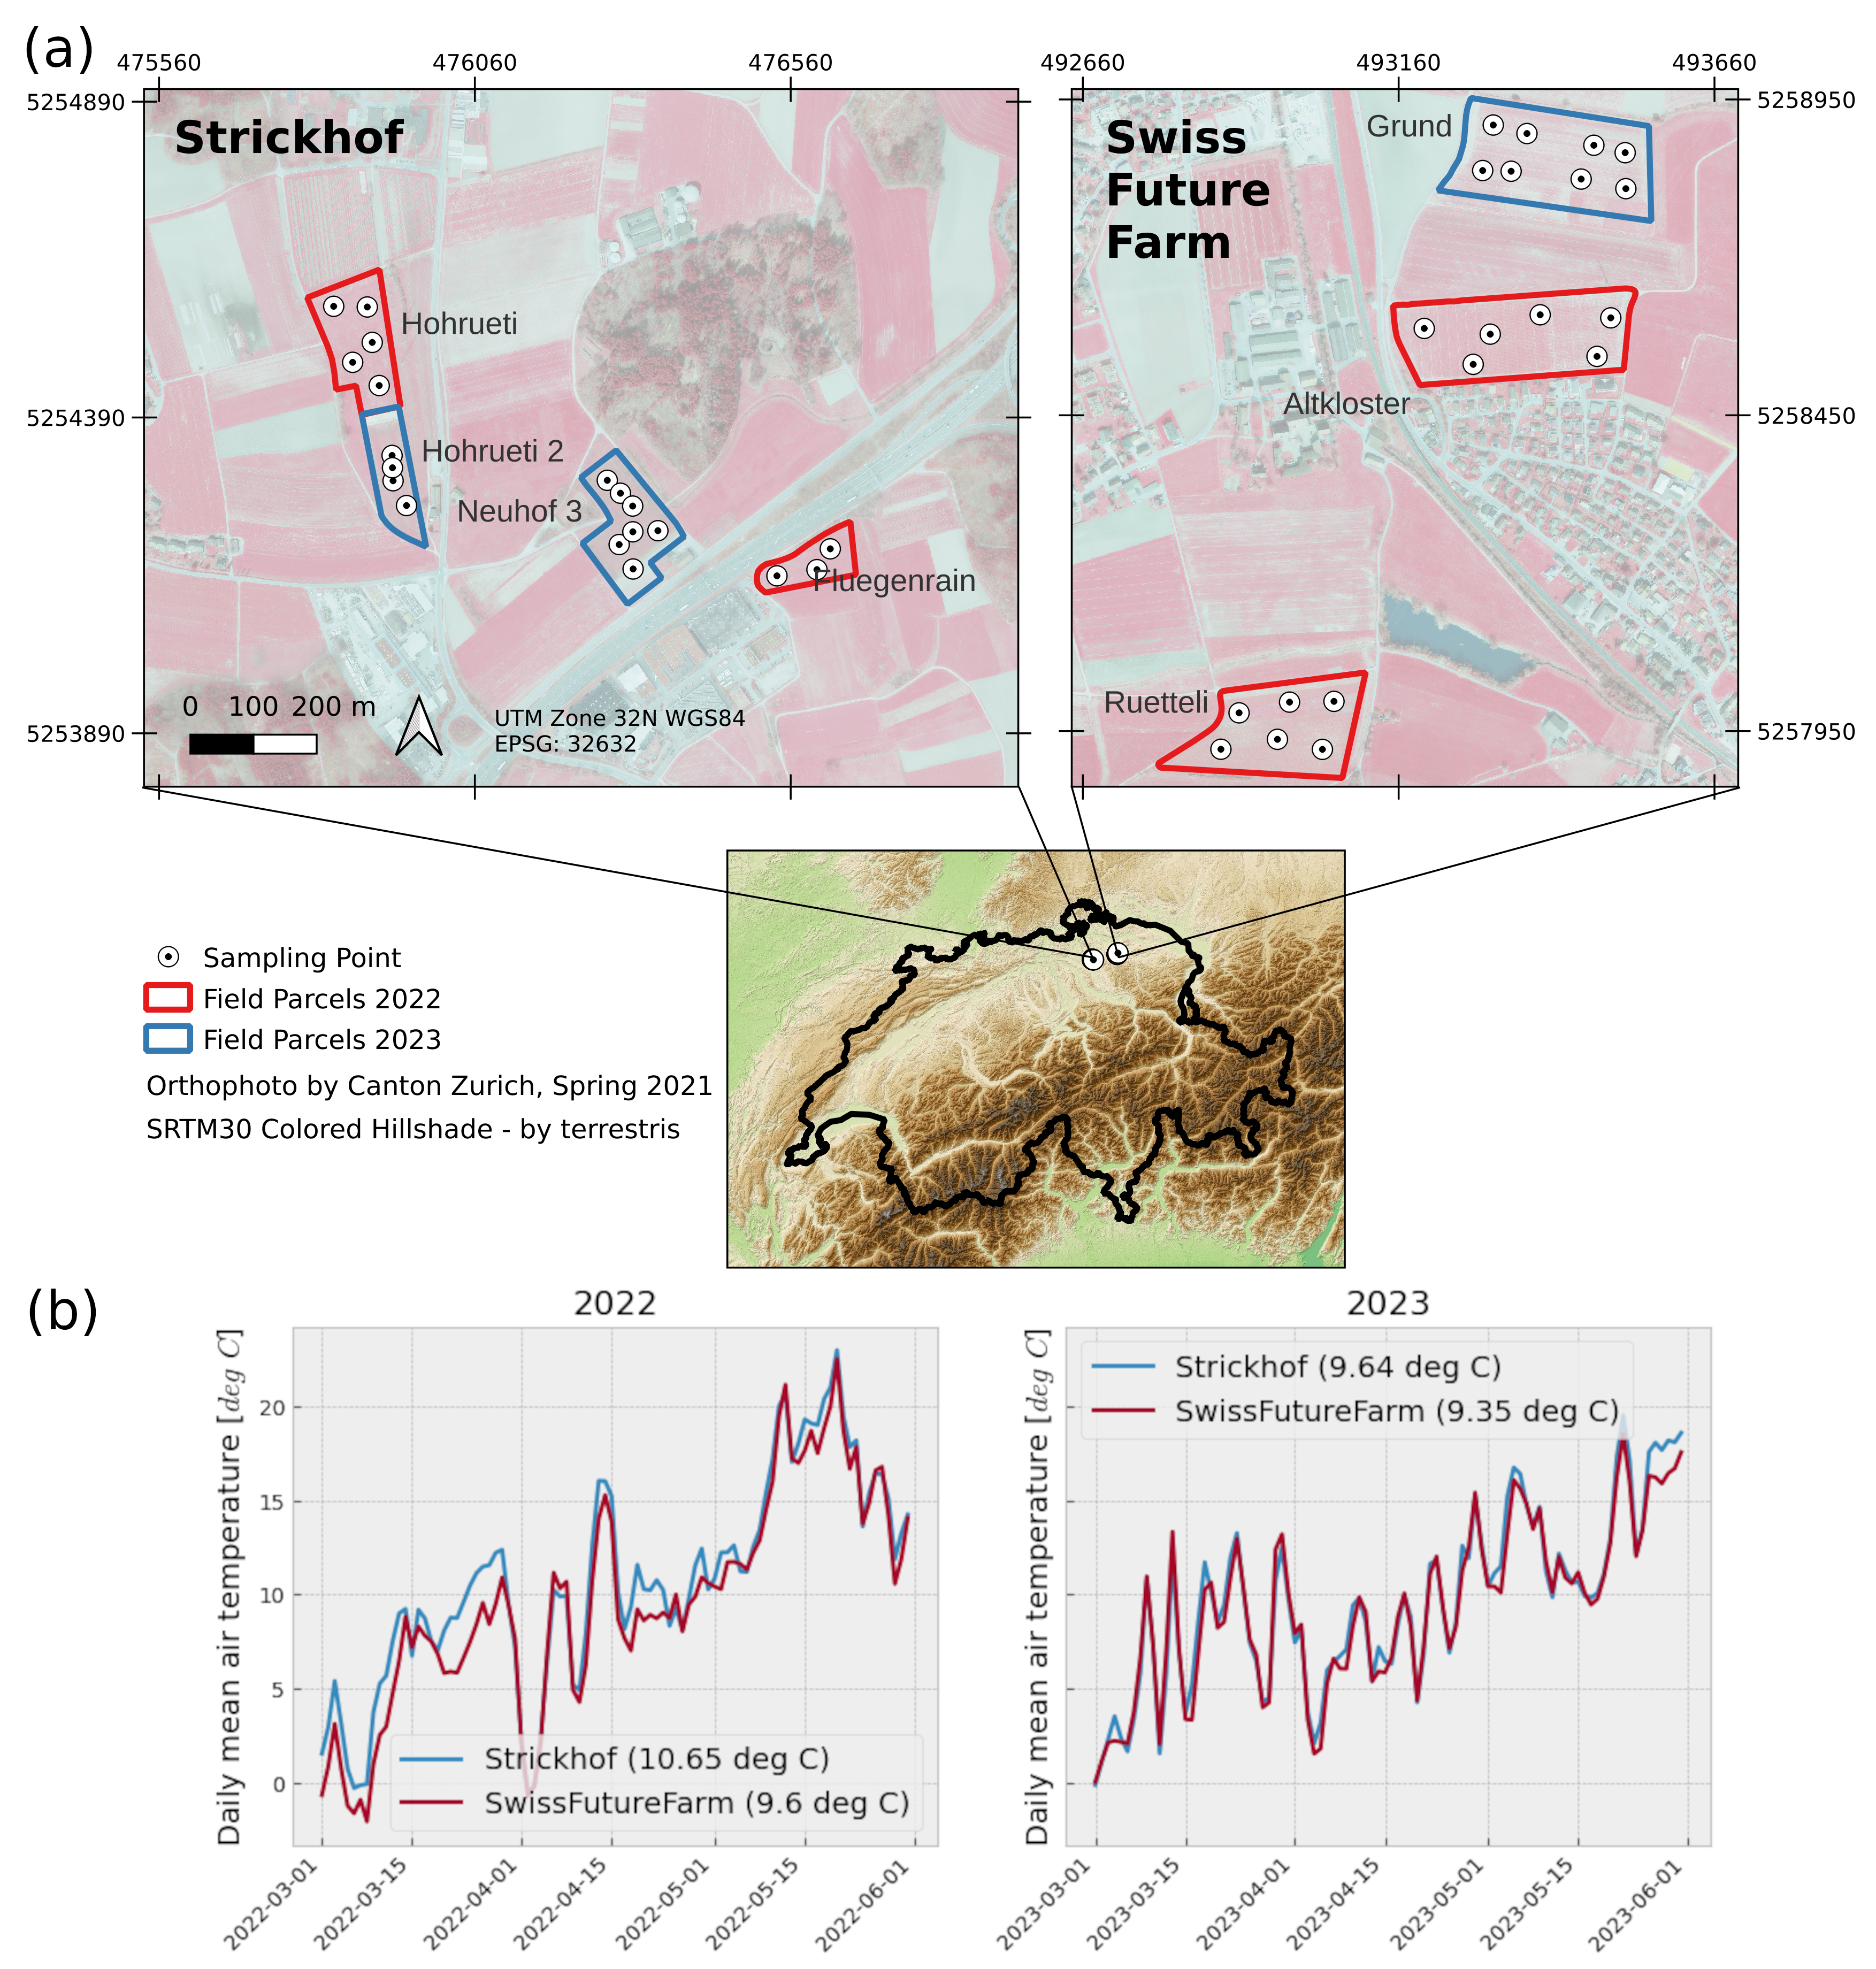
\includegraphics[width=1.0\textwidth]{overview_validation_sites_and_meteo.png}
    \caption{(a) Map of the two sites at which independent validation data was acquired in 2022 (red) and 2023 (blue). Dots denote the position of the sampling points in the field parcels to capture field heterogeneity. (b) Daily mean air temperature 2 m above ground at the validation sites in spring 2022 (left) and 2023 (right). The mean air temperature between 1st of March and 30th of June is given in the legend in brackets.}
    \label{fig:map-validation-sites}
\end{figure}

In terms of meteorology, 2022 and 2023 were different: 2022 had a dry and warm spring, while April and May of 2023 were rainy and higher temperatures only occurred towards the end of May. Figure~\ref{fig:map-validation-sites}b shows the daily mean air temperatures for the Strickhof (blue) and Swiss Future Farm (red) sites in 2022 (left) and 2023 (right). In both years the Strickhof site was warmer than the Swiss Future Farm site. In 2022, the mean air temperature between the beginning of March and June was 10.65 and 9.6 degrees C for Strickhof and Swiss Future Farm, respectively. In 2023 this value decreased to 9.64 and 9.35 degrees C respectively.

\subsection{Sentinel-2 Imagery}
\label{subsec:s2-imagery}
Thanks to its twin-constellation of \gls{S2}A and B, the \gls{S2} platform provides high revisit rates (<= 5 days in mid-latitudes) and captures spectral reflectance data in 13 channels between 490 and 2200 nm in up to 10 m spatial resolution. \gls{S2} has therefore proven an invaluable data source for vegetation studies including the retrieval of crop functional traits~\citep[for instance]{amin_prototyping_2021,delloye_retrieval_2018}.

We obtained \gls{S2} bottom-of-atmosphere (processing level: L2A) imagery from Microsoft Planetary Computer\footnote{\url{https://planetarycomputer.microsoft.com/}} using the open-source Python library EOdal~\citep{graf_eodal_2022} (version 0.2.1; Python 3.10). The data cover the validation sites (Figure~\ref{fig:map-validation-sites}). We used all scenes in 2022 and 2023 between the beginning and ending of the stem elongation phase (i.e., April to June) with a scene-wide cloud cover threshold of $\le$ 50\%. We determined the date range considered per parcel from the in-situ ratings of phenology (Section~\ref{subsubsec:phenology-processing}). In addition, we used a scene before and after the determined time period to provide enhanced temporal context and account for uncertainty regarding the exact onset of the phenological development stages. In total, 17 \gls{S2} scenes were available at the Strickhof site in 2022 and 14 in 2023, while at the Swiss Future Farm site 14 and 11 scenes could be used in 2022 and 2023, respectively.


\section{Methods}
\label{sec:drc_methods}
Figure \ref{fig:workflow-glai-time-series} shows the proposed workflow. Based on in-situ \gls{GLAI} (\textit{"in-situ GLAI"}) values and air temperature data at the calibration sites (Section \ref{subsec:calibration-data}), \gls{DRC}s are fitted and used to model growth rates in hourly and daily resolution (Figure~\ref{fig:workflow-glai-time-series}a). \gls{S2} \gls{GLAI} (\textit{"raw GLAI"}) observations at the validation sites (Section \ref{subsec:validation-data}, Figure \ref{fig:workflow-glai-time-series}b) are assimilated into the \gls{DRC}-based growth curves and used to reconstruct the \gls{GLAI} time series (\textit{"DRC GLAI"}) (Figure \ref{fig:workflow-glai-time-series}c). In addition, a baseline is fit based solely on \gls{S2} \gls{GLAI} observations (\textit{"baseline GLAI"}) using a sigmoid function (Figure \ref{fig:workflow-glai-time-series}d). In a last step, the reconstructed \gls{GLAI} time series are compared to in-situ validation data. The term "coarse spatial resolution", as depicted in Figure \ref{fig:workflow-glai-time-series}, indicates that the meteorological data offered only one reading for each field parcel, without accounting for any within-field variability. On the other hand, high spatial resolution implies that the spatial intricacies regarding within-field heterogeneity are taken into account. Code and data necessary to reproduce all processing and analysis are available under GNU General Public License v3.0\footnote{\url{https://github.com/EOA-team/sentinel2_crop_trait_timeseries}}. The methods section follows this structure and starts with the processing of the in-situ data.

\begin{figure}[H]
    \centering
    \includegraphics[width=1.0\textwidth]{06-DRC/img/workflow_glai_ts_reconstruction.pdf}
    \caption{Proposed workflow to reconstruct continuous \gls{GLAI} time series with high spatial and temporal resolution using temperature-based \gls{DRC}s to obtain \gls{GLAI} growth rates (a), \gls{S2} raw \gls{GLAI} observations per pixel (b) and data assimilation and \gls{DRC}-based interpolation of assimilated \gls{DRC} \gls{GLAI} values (c). The baseline method using a sigmoid function fit to the \gls{S2} \gls{GLAI} data (baseline \gls{GLAI}) is shown in (d).}
    \label{fig:workflow-glai-time-series}
\end{figure}

\subsection{Processing of in-situ data}
Throughout the main growing season of winter wheat (beginning of March till end of June in central Europe) continuous, mostly weekly measurements of \gls{GLAI} and phenology were undertaken at the calibration (Section~\ref{subsec:calibration-data}) and validation sites (Section~\ref{subsec:validation-data}). All measurements were linked to hourly air temperature readings 2 m above ground available from nearby weather stations.

\subsubsection{Air temperature data}
Air temperature data was acquired hourly 2 m above ground in deg C. In addition, the temperature readings were aggregated to daily resolution by averaging all 24 hourly measurements of a day from midnight to midnight.

\subsubsection{Green Leaf Area Index}
\label{subsubsec:glai-processing}
\gls{GLAI} samples were derived non-destructively using a LAI-2200C Plant Canopy Analyzer by LI-COR Biosciences with a 45 degree viewing cap. Measurements were performed at pre-defined sampling points within the fields (see, e.g., Figure~\ref{fig:map-validation-sites}a). For each measurement, three replicates were performed in different orientations each of them offset by 90 degrees. To avoid contamination of the measurement by direct sun light the measurements were either shaded manually, taken under diffuse light conditions (over-cast sky, fog) or acquired early in the morning.

\subsubsection{Phenology}
\label{subsubsec:phenology-processing}
Estimates of \gls{GLAI} (Section~\ref{subsubsec:glai-processing}) were linked to phenological development.
Phenological development of the winter wheat canopies was expressed in \gls{BBCH} scale following~\cite{lancashire_uniform_1991}. For the rating of the beginning of stem elongation (BBCH 30) we cut the main tiller lengthwise and measured the distance between the first node and the tillering node following the manual by~\cite{pask_physiological_2012}. End of heading (BBCH 59) was reached when the inflorescence was fully emerged.

\subsection{Model calibration to introduce physiological knowledge}
\label{subsec:model-cal}

Model calibration introduces the a-priori physiological knowledge about the relationship between plant growth and air temperature (Figure \ref{fig:workflow-glai-time-series}a). The knowledge was based on a dataset of in-situ \gls{GLAI} measurements from the calibration sites (Section~\ref{subsec:calibration-data}). The measured in-situ \gls{GLAI} values were used to calculate \gls{deltaGLAI} between two time points, which represent increase, respectively growth of the wheat canopy (Equation~\ref{eq:delta_LAI}) (as in \cite{tschurr_frost_2023}). In-situ \gls{GLAI} values have been smoothed using cubic smoothing splines before the calculation of \gls{deltaGLAI}.

\begin{equation}
\label{eq:delta_LAI}
  \Delta GLAI(t_n) =  GLAI(t_{n}) - GLAI(t_{n-1})\,,
\end{equation}

The \gls{deltaGLAI} value can then be expressed using the temperature trajectory between time point t\textsubscript{n} and t\textsubscript{n-1} in either hourly or daily granularity.

\subsubsection{Fitting of Dose-Response Curves}
\label{subsubsec:fitting-drc}
% DRCs
The calibration dataset was utilised to optimise three distinct \gls{DRC}, as illustrated in Figure~\ref{fig:DRC_overview}. Each curve represents the behaviour of the \gls{deltaGLAI} as a function of the observed temperature. The simplest \gls{DRC} displays a non-linear correlation between growth and temperature, with zero growth deemed below $T_{base}$. A linear growth reaction is projected for temperatures exceeding $T_{base}$. We hereafter refer to this growth response curve as the non-linear DRC (e.g., as seen in \cite{roth_field_2023}). Additionally, an asymptotically shaped DRC was employed, accounting for a base temperature ($T_{base}$), below which no growth occurs. Above $T_{base}$, the DRC exhibits a maximum growth response, defined by the curve's asymptote, along with the parameter lrc, allowing for an asymptotic shape of the curve (e.g., see \cite{roth_phenomics_2022}). Similar to the asymptotic \gls{DRC}, the Wang Engels \gls{DRC} can be defined by three parameters: $T_{base}$, which is the temperature below which growth does not occur, $T_{opt}$, which defines the highest growth rate response, and $T_{max}$, which is the temperature above which the growth rate is set to zero~\citep{wang_simulation_1998, wang_uncertainty_2017} (refer to Figure~\ref{fig:DRC_overview}).

\begin{figure}[H]
    \centering
    \includegraphics[width=0.8\textwidth]{06-DRC/img/DRC_curves_scheme.png}
    \caption{Schematic overview of the three used dose response curves (DRC), non linear, asymptotic and Wang Engels curve. The x axis represents the input temperature, the y axis the corresponding response in green leaf area index (GLAI) growth.}
    \label{fig:DRC_overview}
\end{figure}


\begin{table}[H]
\caption{Dose response curve parameters and constraints used for model fitting.}
\label{tab:drc_fitting}
\centering
\begin{tabular}{lll}
\toprule
\textbf{Dose response curve} & \textbf{parameters}    & \textbf{constraints}                          \\ \hline
non linear          & $T_{base}$ , slope         &                                      \\
asymptotic          & $T_{base}$, lrc, asymptote & $T_{base}$ \textless asymptote \\
Wang Engels &
  \begin{tabular}[c]{@{}l@{}} $T_{base}$,\\  $T_{opt}$,\\   $T_{max}$\end{tabular} &
  \begin{tabular}[c]{@{}l@{}} $T_{base}$\\  \textless $T_{opt}$ \\ \textless  $T_{max}$\end{tabular}
\\
\bottomrule
\end{tabular}
\end{table}

% fitting nloptr
The parameters for each of the three \gls{DRC}s (refer to Table~\ref{tab:drc_fitting}) were optimised utilising the calibration data explained earlier. An augmented Lagrangian algorithm employing the nloptr package in R \citep{rcore-team_r_2014,johnson_nlopt_2007} was used for this purpose. Regarding our third research question, optimisation was conducted for temperature values of both hourly and daily measurements.

As the curves used can solely depict ascending \gls{GLAI} values, we excluded negative \gls{deltaGLAI} values prior to optimization. These values are typically attributable to measurement uncertainty and imprecisions, such as those related to sensor positioning. As a result, 20\% of \gls{deltaGLAI} values were rejected. Constrained optimization by linear approximation (COBYLA) was used as the local solver for optimization, providing upper and lower bounds and a starting value \citep{powell_direct_1994}. Initial values were determined either by quantile values of input temperature data (for $T_{base}$, $T_{opt}$, and $T_{max}$) or by empirically derived values (slope, lrc, and asymptote) (refer to Table \ref{tab:Sup_starting_paramters} in the Appendix). Optimisation was carried out 20 times on a randomly selected 80\% of the data, and the final parameters were derived from the median of the 20 subset optimisations to obtain more robust parameter values, thereby reducing the possible influence of outliers. For each temperature measurement, the corresponding dose response value was calculated and accumulated over time. To optimise the parameters, the \gls{RMSE} between these accumulated values and the \gls{deltaGLAI} measurements was minimised. The skill score was negatively impacted for meeting constraints (Table~\ref{tab:drc_fitting}) or for forecasting \gls{deltaGLAI} values that were too low to attain physiologically significant parameter and prediction values.

\subsection{Processing of \gls{S2} data}

\gls{S2} raw \gls{GLAI} observations introduce spatial detail (Figure \ref{fig:workflow-glai-time-series}b).
We used all 10 and 20 m bands except band 8 (central wavelength 842 nm). Band 8 was discarded in favor of band 8A (central wavelength 865 nm) which provides a higher spectral resolution than band 8. Thus, nine bands between 492 and 2200 nm were used: B2 (blue), B3 (green), B4 (red), B5 (red-edge 1), B6 (red-edge 2), B7 (red-edge 3), B8A (near-infrared 2), B11 (shortwave-infrared 1), and B12 (shortwave-infrared 2). See also Table \ref{tab:s2-bands} in the Appendix for details about the native spatial resolution, spectral band widths and central wavelengths of these bands.

First, we clipped the \gls{S2} data to the spatial extent of the field parcels at the validation sites (Figure~\ref{fig:map-validation-sites}a). Next, we resampled the six 20 m bands (see Table \ref{tab:s2-bands}) to a spatial resolution of 10 m using nearest neighbor interpolation.

All scenes were pre-processed by ESA using the payload data ground segment (PDGS) baselines 4.00 (2022 data) and 5.09 (2023 data) that compromise an improvement radiometric harmonization of S2A and S2B as well as geometric refinements that fulfil the CEOS Analysis Ready Data for Land (CEOS ARD) standard. Therefore, no further refinements such as image co-registration were undertaken.

\subsubsection{Data cleaning}
We used the \gls{SCL} delivered as part of the \gls{S2} L2A product to filter out clouds, shadows, open water, snow and cirrus on a per-pixel basis. Thus, only the SCL classes 4 (vegetation) and 5 (bare soil) were kept. Pixel values with a different \gls{SCL} class assignment were masked and not considered any further.

\subsubsection{Radiative transfer modelling}
To extract raw \gls{GLAI} from \gls{S2} scenes at the validation sites (Section~\ref{subsec:s2-imagery}) we used the four-stream \gls{RTM} PROSAIL~\citep{jacquemoud_prospectsail_2009} to simulate bi-directional reflectance factors of winter wheat canopies. PROSAIL couples the leaf \gls{RTM} PROSPECT-D~\citep{feret_prospect-d_2017} with the canopy \gls{RTM} 4SAIL~\citep{verhoef_light_1984}. We parameterized the \gls{RTM} inputs to reflect typical physiological and morphological characteristics of winter wheat canopies between \gls{BBCH} stages 30 and 59 based on a comprehensive field phenotyping dataset described in \cite{graf_insights_2023}. The leaf (PROSPECT-D) and canopy (4SAIL) input parameters including their range and distribution are shown in Table~\ref{tab:drc-prosail-inputs} based on \cite{graf_insights_2023}. Following the proposed workflow by \cite{graf_insights_2023} we increased the physiological plausibility of \gls{RTM} inputs. In detail, the leaf chlorophyll a+b and leaf carotenoid content were re-distributed based on empirical relationships between these traits and the \gls{GLAI} established in \cite{graf_insights_2023} (GLAI - Cab relationship) and \cite{wocher_rtm-based_2020} (Cab - Car relationship). Using these relationships we can re-distribute Cab (through the canopy chlorophyll content) solely based on \gls{GLAI}. Similarly, Car can be re-distributed solely based on Cab obtained in the previous step.

We run PROSAIL in forward mode based on the input parameters denoted in Table~\ref{tab:drc-prosail-inputs} for each \gls{S2} scene during the stem elongation period. Illumination and observer angles were set to scene-specific values obtained from the \gls{S2} scene metadata. In total, we run 50 000 PROSAIL simulations per \gls{S2} scene. The resulting spectra were converted to the spectral resolution of \gls{S2} by convolution of the original PROSAIL outputs in 1 nm spectral resolution with the spectral response functions of \gls{S2}A and B provided by ESA\footnote{\url{https://sentinel.esa.int/web/sentinel/user-guides/sentinel-2-msi/document-library/-/asset_publisher/Wk0TKajiISaR/content/sentinel-2a-spectral-responses}}. In addition, we applied further physiological plausibility checks introduced by~\cite{wocher_rtm-based_2020}. In detail, we dropped simulated spectra with a shift of the green reflectance peak towards wavelengths shorter than 574 nm, which was considered implausible based on extensive survey of handheld and airborne hyperspectral imaging data of green vegetation. Around 10\% of the simulated PROSAIL spectra were therefore discarded. The resulting spectra were stored in lookup tables (\gls{LUT}s) per \gls{S2} scene.

\begin{table}[H]
\centering
\caption{Parameter ranges and distributions for the combined leaf (PROSPECT-D) and canopy (4SAIL) \gls{RTM} (PROSAIL) for winter wheat canopies in the stem elongation phase. The ranges are given for uniform distributions (range) or a truncated Gaussian distribution with mean and standard deviation denoted in brackets. Cab and Car are redistributed on \gls{GLAI}. All values and distributions are taken from \cite{graf_insights_2023}.}
\label{tab:drc-prosail-inputs}
\begin{tabular}{@{}lllllll@{}}
\toprule
  \textbf{Trait}     & \textbf{Description}         & \textbf{Unit}           & \multicolumn{4}{l}{\textbf{Range}}              \\ \midrule
\multicolumn{7}{l}{\textbf{PROSPECT-D (Leaf)}}                                                                \\
\midrule
N      & Leaf Structure Parameter     & {[}-{]}                 & \multicolumn{4}{l}{1 - 2.5 (1.5, 0.2)}          \\
Cab    & Leaf Chlorophyll a+b Content & {[}$\mu g$ $cm^{-2}${]} & \multicolumn{4}{l}{redistributed based on GLAI} \\
Car    & Leaf Carotenoid Content      & {[}$\mu g$ $cm^{-2}${]} & \multicolumn{4}{l}{redistributed based on Cab}  \\
Cant   & Leaf Anthocyanin Content     & {[}$\mu g$ $cm^{-2}${]} & \multicolumn{4}{l}{0.0 - 5.0 (2.0, 0.8)}        \\
Cbrown & Brown Pigments               & {[}-{]}                 & \multicolumn{4}{l}{0 - 1}                       \\
Cw     & Equivalent Water Thickness   & {[}cm{]}                & \multicolumn{4}{l}{0 - 0.07 (0.04, 0.02)}       \\
Dm     & Dry Matter Content           & {[}$g$ $cm^{-2}${]}     & \multicolumn{4}{l}{0 - 0.01}                    \\
\midrule
\multicolumn{7}{l}{\textbf{4SAIL (Canopy)}}                                                                     \\
\midrule
GLAI   & Green Leaf Area Index        & {[}$m^2$ $m^{-2}${]}    & \multicolumn{4}{l}{0.5-6.5}                         \\
ALA    & Leaf Inclination Angle       & {[}deg{]}               & \multicolumn{4}{l}{30 - 70}                     \\
hspot  & Hot spot Parameter           & {[}-{]}                 & \multicolumn{4}{l}{0.01 - 0.5}                  \\
rsoil  & Soil Brightness Factor       & {[}-{]}                 & \multicolumn{4}{l}{0 - 1}                       \\
psoil  & Dry/ Wet Soil Factor         & {[}-{]}                 & \multicolumn{4}{l}{0 - 1}                       \\ \bottomrule
\end{tabular}
\end{table}


\subsubsection{Radiative transfer model inversion}
\label{subsubsec:rtm-inv}
For \gls{RTM} inversion we used the PROSAIL spectra stored in \gls{LUT}s per scene. We retrieved raw \gls{GLAI} per \gls{S2}  pixel by comparing \gls{S2}-observed ($\rho_{S2}$) spectra with the simulated spectra in the \gls{LUT} ($\rho_{LUT}$) by means of the \gls{MAE} for all $n$ \gls{S2}-bands considered (i.e., $n=9$) as suggested by \cite{graf_insights_2023}.

\begin{equation}
    MAE = \frac{1}{n} \sum_{i=0}^{n} |\rho_{{S2}_i} - \rho_{{LUT}_i} |
\end{equation}
The median \gls{GLAI} value obtained from the 5000 simulated spectra with the smallest \gls{MAE} was then used as the \gls{S2}-derived raw \gls{GLAI} observation per \gls{S2} pixel.


\subsection{Time series reconstruction}
\label{subsec:drc-model-inference}

\subsubsection{DRC-derived growth rates at the farm scale}

Fitted \gls{DRC}s were applied to hourly and daily air temperature data at the validation sites (Section~\ref{subsec:validation-data}, Figure \ref{fig:workflow-glai-time-series}a). This converted each air temperature reading into a \gls{GLAI} growth rate. Thus, per site and \gls{DRC} \gls{GLAI} growth rates in hourly and daily resolution were available.

\subsubsection{S2-derived raw GLAI observations at the pixel scale}
\label{subsubsec:s2-glai-simple-outlier-filter}
A simple outlier detection formalism was introduced to account for undetected atmospheric disturbances in the raw \gls{S2} \gls{GLAI} observations (Figure \ref{fig:workflow-glai-time-series}b). Atmospheric disturbances usually cause negatively biased outliers in remotely-sensed trait observations~\citep{chen_simple_2004}. Therefore, raw \gls{S2} \gls{GLAI} values of a pixel that deviated from the mean of all raw \gls{GLAI} values by more than a single standard deviation in the negative y-direction were discarded. This did not apply to the first \gls{GLAI} observation in time due to two reasons: First, we lack sufficient temporal context. Second, due to its proximity to the early phase of stem elongation a low \gls{GLAI} value is physiologically plausible.

\subsubsection{Data assimilation using Ensemble Kalman Filtering}
We aimed to combine the modelled \gls{DRC} \gls{GLAI} growth rates reflecting a-priori physiological knowledge about the relationship of growth to air temperature with raw \gls{S2} \gls{GLAI} observations to obtain the best possible estimate of the effective \gls{GLAI} (Figure \ref{fig:workflow-glai-time-series}c). Combining models with observations presents a data assimilation problem. In our case, we assimilated the raw \gls{S2} \gls{GLAI} observations into the \gls{DRC}-based \gls{GLAI} growth rates to introduce spatial detail while retaining the high temporal resolution and physiological meaning of the underlying temperature data.

For data assimilation, the \gls{KF} is widely used. In essence, \gls{KF} is a sequential approach estimating the "true", hidden state vector of a system by updating the modelled states whenever an observation becomes available. In our case, the hidden state vector is given by the actual but unknown \gls{GLAI} time series of a pixel. Since, both, the \gls{DRC} models and the \gls{S2} observations have uncertainties, we use the probabilistic \gls{EnsKF}. The \gls{EnsKF} allows to include model and observation uncertainty into the data assimilation process~\citep{evensen_ensemble_2003}. \gls{EnsKF} frameworks have therefore been widely used in assimilating remotely sensed crop traits in crop models~\citep{de_wit_crop_2007, zhao_assimilating_2013, huang_assimilating_2016}. ~\cite{graf_propagating_2023} found that raw \gls{GLAI} values derived from \gls{S2} take relative standard uncertainties up to 5\% due to uncertainty in the \gls{S2} top-of-atmosphere reflectance data. For in-situ \gls{GLAI} and temperature data we estimated a similar magnitude of uncertainty and set relative model uncertainty to 5\%. The \gls{EnsKF} ensemble size was set to 50 ensemble members to balance computational complexity with statistical significance as suggest by ~\cite{de_wit_crop_2007} and ~\cite{zhao_assimilating_2013}.

Figure~\ref{fig:assimilation-sample-pixel} shows the proposed data assimilation approach, i.e., a zoom-in into Figure~\ref{fig:assimilation-sample-pixel}c, for a randomly selected \gls{S2} pixel at the Strickhof site in 2022. Figure \ref{fig:assimilation-sample-pixel}a denotes the hourly air temperature time series available from the nearby weather station that was input into the \gls{DRC}s to obtain hourly \gls{GLAI} growth rates. The raw \gls{S2} \gls{GLAI} observations (red dots) were assimilated into the \gls{DRC} \gls{GLAI} growth rates (Figure \ref{fig:assimilation-sample-pixel}b) and subsequently used to reconstruct the final \gls{DRC} \gls{GLAI} time series with uncertainties (Figure \ref{fig:assimilation-sample-pixel}c). Below we explain the steps in more detail.

\begin{figure}[H]
    \centering
    \includegraphics[width=\textwidth]{06-DRC/img/interpolated_lai_5255495.0_475965.0_hourly.png}
    \caption{Example of the proposed probabilistic \gls{GLAI} assimilation for a single \gls{S2} pixel at the Strickhof site in 2022 combining hourly air temperature data (a) with raw \gls{S2} \gls{GLAI} observations (red dots) using \gls{DRC}-based cumulative daily growth rates (solid colored lines in b) to reconstruct \gls{GLAI} time series with associated uncertainties (c). The dose-response curve type used in this case was asymptotic.}
    \label{fig:assimilation-sample-pixel}
\end{figure}

As a first step, we performed a conventional \gls{EnsKF} assimilation (Figure~\ref{fig:assimilation-sample-pixel}b) using \gls{DRC}-based growth rates derived from air temperature time series (Figure~\ref{fig:assimilation-sample-pixel}a). As the \gls{DRC}s provide growth rates, an initial \gls{GLAI} must be provided. We therefore initialised each of the 50 ensembles by randomly sampling between the lower and upper \gls{GLAI} bounds using a uniform probability distribution. The initial \gls{GLAI} bounds were set to a range of 0.5 to 1.5$m^2$ $m^{-2}$ based on empirical knowledge. We started the model runs just before the first \gls{S2} observation (Figure~\ref{fig:assimilation-sample-pixel}b, left). We then accumulated all the \gls{DRC} \gls{GLAI} growth rates up to the first raw \gls{S2} \gls{GLAI} observation. At the time $t$ of the observation, we computed the Kalman gain $K$:

\begin{equation}
\label{eq:kalman-gain}
    K = P_e H^T (H P_e H^T + R_e)^{-1}
\end{equation}
In Equation~\ref{eq:kalman-gain}, $P_e$ and $R_e$ denote the model and observation covariance matrices based on their uncertainties, and $H$ is the measurement operator which is the identity matrix since \gls{GLAI} is directly observable. Using $K$, we calculate the Kalman innovation term $KI$

\begin{equation}
    KI = D - (H A)
\end{equation}
where $D$ denotes the observation matrix with uncertainties and $A$ is the matrix with modelled \gls{GLAI} values at time $t$. Thus, the model state at the analyses step $A^a$ can be obtained:

\begin{equation}
\label{eq:kalman-analyses-step}
    A^a = A + K\ KI
\end{equation}
$A^a$ re-initializes the ensembles at $t$. As before, we then calculated the cumulative \gls{DRC} growth rates until the next raw \gls{S2} \gls{GLAI} observation at time $t+1$. At $t+1$ a new $A^a$ was calculated using Equations~\ref{eq:kalman-gain} to~\ref{eq:kalman-analyses-step}. This procedure was repeated for all \gls{S2} observations except the last one as shown in Figure~\ref{fig:assimilation-sample-pixel}b.

Here, a limitation of the \gls{EnsKF} method becomes clear: \gls{EnsKF} is a non-conservative approach, i.e., potentially large jumps in the modeled time series are caused by the assimilation (Figure~\ref{fig:assimilation-sample-pixel}b). This is physiologically implausible, since GLAI trajectories must be continuous. Therefore, we had to extended the EnsKF approach in a second step:

We addressed said problem by replacing the raw \gls{S2} \gls{GLAI} observations with the ensemble mean at each analysis step $A^a$ ($GLAI_{assim}$). This is to ensure that model and observation information is preserved. The ensemble standard deviation is retained as a measure of uncertainty, taking into account both, model and observation uncertainty. Using the $GLAI_{assim}$ values, we used the \gls{DRC}s for a second time to model growth. This time, however, we used the \gls{DRC}s to interpolate between the $GLAI_{assim}$ values, which are still temporally sparse. We scaled the cumulative growth rates to exactly match the $GLAI_{assim}$ values. In case $GLAI_{{assim}_{t+1}}$ was smaller than $GLAI_{{assim}_{t}}$, $GLAI_{{assim}_{t+1}}$ was discarded. In this case, we interpolated between $GLAI_{{assim}_t}$ and $GLAI_{{assim}_{t+2}}$. This ensured that undetected outliers in the raw \gls{S2} \gls{GLAI} values were not given too much weight, while preserving medium range temporal characteristics. The resulting interpolated \gls{GLAI} curve at the temporal resolution of the \gls{DRC} (i.e., hourly or daily) is shown in Figure~\ref{fig:assimilation-sample-pixel}c, in which the solid blue line denotes the assimilated, \gls{DRC}-interpolated reconstructed \gls{GLAI} time series.

From here on we name the reconstructed time series after the underlying \gls{DRC}s. That is, by "non linear" we mean from now on the \gls{EnsKF} assimilated and interpolated data points created using the non linear \gls{DRC} and raw \gls{S2} \gls{GLAI} observations. The same applies to "asymptotic" and "Wang Engels".

\subsubsection{Baseline method}
\label{subsubsec:baseline-method}
As baseline method, a sigmoid (a.k.a. logistic) function was fitted to the same raw \gls{S2} \gls{GLAI} observations at the pixel scale (Figure~\ref{fig:workflow-glai-time-series}d). Due to its S-shaped form, sigmoid functions are widely used in remote sensing to obtain continuous time series of vegetation traits. The sigmoid function is a simplified version of \gls{DL}~\citep{beck_improved_2006}, which only accounts for the generative (ascending) branch of \gls{GLAI} development. It is therefore a baseline that, unlike other statistical models such as the Savitzky-Golay filter, already has parameters with a certain biological significance.

The sigmoid function takes four parameters: The supremum of the function's values $L$, the growth rate $k$, the function's midpoint $x_0$ and an offset from zero $b$ which is necessary because \gls{GLAI} values around \gls{BBCH} 30 are usually larger than zero:

\begin{equation}
\label{eq:logistic-function}
    f(x) = \frac{L}{1 + e^{-k(x-x_0)}} + b
\end{equation}

A minimum of four raw \gls{S2} \gls{GLAI} observations are required to fit the model parameters. We fit the sigmoid function to each pixel, taking into account all available \gls{GLAI} observations, using the Levenberg-Marquardt algorithm available in the scipy Python library (version 1.11.0) with the function "scipy.optimze.curve\_fit". The maximum number of optimisation steps was set to 1000. The parameterised logistic function (equation~\ref{eq:logistic-function}) was then used to reconstruct the \gls{GLAI} time series at daily resolution. We will refer to this time series as the baseline \gls{GLAI}.

\subsection{Model Validation}

The raw \gls{S2} \gls{GLAI} observations and the reconstructed continuous \gls{DRC} and baseline \gls{GLAI} time series were compared against the independent in-situ validation \gls{GLAI} data (Section~\ref{subsec:validation-data}). We obtained matching tuples of reconstructed and in-situ \gls{GLAI} by time stamp and spatial intersection of the sampling points with the \gls{S2} 10 m pixel grid. In the case of the reconstructed time series (i.e., \gls{DRC} and baseline \gls{GLAI}), each in-situ \gls{GLAI} value could be matched to a modelled \gls{GLAI} value as the time series is continuous and spans the whole time period for which in-situ data was available. For the raw \gls{S2} \gls{GLAI} observations this was not the case due to the aforementioned temporal sparsity of the satellite observations. Therefore, we only used in-situ \gls{GLAI} values that had a satellite overpass with a maximum difference of one day.

Comparison was carried out by means of common error measures of the linear regression between modelled and observed values. Error measures included the \gls{RMSE}, \gls{nRMSE}, \gls{R2}, and bias between reconstructed ($GLAI_{reconstructed}$) and in-situ \gls{GLAI} values ($GLAI_{insitu}$). The bias was calculated using the variance of $GLAI_{reconstructed}$ ($var(GLAI_{reconstructed})$) and the mean of the squared differences ($MSD$) between mean $GLAI_{reconstructed}$, $\mu(GLAI_{reconstructed})$, and $GLAI_{insitu}$ considering all $n$ matching tuples available:

\begin{equation}
    MSD = \frac{1}{n} \sum_{i=0}^{n} (\mu(GLAI_{reconstructed}) - GLAI_{{insitu}_i})^2
\end{equation}
\begin{equation}
    Bias = MSD - var(GLAI_{reconstructed})
\end{equation}

Error statistics were produced for all sites and years as well as for single sites, years and \gls{BBCH} macro stages (i.e, \gls{BBCH} 30-39, 50-59) to assess model performance in space, time, and with respect to phenological development. In addition, we visualized the temporal trajectories of \gls{GLAI} per parcel to evaluate the physiological plausibility and consistency of the reconstructed \gls{GLAI} time series.


\section{Results}
\label{sec:drc_results}
\subsection{Validation of raw S2 GLAI observations against in-situ GLAI}

Figure \ref{fig:s2-obs-scatter-plots} shows the raw \gls{S2} \gls{GLAI} observations plotted against in-situ measured \gls{GLAI} with a maximum temporal offset of one day. The \gls{RMSE} was about 1.16 $m^2$ $m^{-2}$ (\gls{nRMSE} 18.92\%) with a bias of 1.87 $m^2$ $m^{-2}$. The raw \gls{S2} \gls{GLAI} observations explained 64\% of the variability in the in-situ values. The raw \gls{S2} \gls{GLAI} values showed a clear underestimation of in-situ \gls{GLAI} > 5 $m^2$ $m^{-2}$ in 2022 (blue dots in Figure \ref{fig:s2-obs-scatter-plots}) as well as three isolated outliers in 2023 (cross markers) for in-situ \gls{GLAI} values between 2 and 3 $m^2$ $m^{-2}$. Due to high cloud cover, only 8 out of 55 available observations for validation were recorded in 2023. Therefore, no year effects could be studied. The same applies to the phenological macro-stages for which not enough data was available to compute robust error statistics.

\begin{figure}[H]
    \centering
    \includegraphics[width=0.6\textwidth]{s2_glai-obs_validation.png}
    \caption{Scatter plots of S2 observed and in-situ measured GLAI at the validation sites using data from 2022 and 2023. The oblique solid lines denotes the desired 1:1 fit; the dashed line denotes the linear regression line between S2 observed and in-situ measured \gls{GLAI} values. N = 55. The years are color-coded.}
    \label{fig:s2-obs-scatter-plots}
\end{figure}

\subsection{Validation of reconstructed GLAI time series against in-situ GLAI}
Similar to Figure \ref{fig:s2-obs-scatter-plots}, scatter plots of reconstructed GLAI (i.e., \gls{DRC} and baseline \gls{GLAI}) at hourly and daily resolution against in-situ measured \gls{GLAI} are displayed in Figure~\ref{fig:glai-scatter-plots} (N = 178). Figure~\ref{fig:glai-scatter-plots} (a-c) shows the results of the proposed \gls{DRC} GLAI time series, and (d) the baseline \gls{GLAI} results which are available in daily resolution, only. The error statistics are listed in Table~\ref{tab:error-stats}.

\begin{figure}[H]
    \centering
    \includegraphics[width=\textwidth]{glai_scatter_plots.png}
    \caption{Scatter plots between reconstructed \gls{DRC} (a-c) and baseline (d) \gls{GLAI} and in-situ \gls{GLAI} at the validation sites using data from 2022 and 2023 (color-coded). For each \gls{DRC} \gls{GLAI}, the results using hourly and daily mean air temperature are shown (a-c). The baseline \gls{GLAI} is only available in daily resolution (d). The oblique solid line denotes the desired 1:1 fit and the dashed line the linear regression line between reconstructed and in-situ \gls{GLAI} values. N = 178.}
    \label{fig:glai-scatter-plots}
\end{figure}

All models revealed a tendency to overestimate low in-situ \gls{GLAI} (< 1.0 $m^2$ $m^{-2}$). The baseline (Figure~\ref{fig:glai-scatter-plots}d) clearly underestimated in-situ \gls{GLAI} values > 5.0 $m^2$ $m^{-2}$. All models performed similar in terms of \gls{RMSE}, \gls{nRMSE} and \gls{R2} (Table~\ref{tab:error-stats}). The hourly asymptotic \gls{DRC} \gls{GLAI} had the smallest \gls{RMSE} (0.98 $m^2$ $m^{-2}$) closely followed by the daily asymptotic and non linear \gls{DRC} \gls{GLAI} (\gls{RMSE} around 0.99  $m^2$ $m^{-2}$, \gls{nRMSE} around 15\%). The highest \gls{RMSE} was observed for the Wang Engels \gls{DRC} \gls{GLAI} at hourly resolution (1.12  $m^2$ $m^{-2}$, \gls{nRMSE}: 17.43\%). The baseline \gls{GLAI} had a slightly lower \gls{RMSE} (1.05  $m^2$ $m^{-2}$, \gls{nRMSE}: 16.27\%) than the daily Wang Engels \gls{DRC} \gls{GLAI} (1.06  $m^2$ $m^{-2}$). A similar picture revealed \gls{R2} which ranged between 0.54 (Wang Engels hourly \gls{DRC} \gls{GLAI}) and 0.70 (non linear daily \gls{DRC} \gls{GLAI}). The highest bias was observed for the baseline \gls{GLAI} (1.66  $m^2$ $m^{-2}$). This was higher than for the \gls{DRC} \gls{GLAI} and more than two times larger than the smallest bias (0.73  $m^2$ $m^{-2}$) obtained from the hourly Wang Engels \gls{DRC} \gls{GLAI} which had the lowest bias.

\begin{table}[H]
\caption{Error statistics of reconstructed and in-situ \gls{GLAI} values (N = 178). \gls{RMSE} and bias are given in $m^2$ $m^{-2}$, \gls{nRMSE} in percent and \gls{R2} is dimensionless.}
\label{tab:error-stats}
\centering
\begin{tabular}{@{}llllll@{}}
\toprule
model                        & resolution & \gls{RMSE}          & \gls{nRMSE}         & Bias          & \gls{R2}            \\ \midrule
\multirow{2}{*}{Non linear} & hourly      & 0.99          &  15.44 & 1.46          & 0.65          \\
                             & daily       & 0.99          & 15.34 & 1.36          & 0.70 \\
\multirow{2}{*}{Asymptotic}  & hourly      & 0.98 & 15.17 & 1.40          & 0.66          \\
                             & daily       & 0.98 & 15.19 & 1.31          & 0.69          \\
\multirow{2}{*}{Wang Engels}  & hourly      & 1.12          & 17.43          & 0.73 & 0.54          \\
                             & daily       & 1.06          & 16.47          & 0.91          & 0.59          \\
Baseline (sigmoid)                      & daily       & 1.05          & 16.27          & 1.66          & 0.66          \\ \bottomrule
\end{tabular}
\end{table}

\subsubsection{Effect of the years}
Error statistics by year are shown in Table~\ref{tab:error-stats-years}. Arrows in table indicate whether a metric value remain unchanged ($\rightarrow$), decrease ($\downarrow$), or increased ($\uparrow$) from 2022 to 2023. For all models and temporal resolutions, the relative error was higher and $R^2$ lower in 2023 (N = 82) than 2022 (N = 96). In 2022, nRMSE values ranged from 13.04 (Wang Engels daily) to 16.72\% (non linear daily), while $R^2$ took values between 0.74 (baseline) and 0.8 (Wang Engels daily). In 2023, nRMSE values were in the range between 17.16 (asymptotic daily) and 25.62\% (Wang Engels hourly) with $R^2$ between 0.3 (Wang Engels hourly) and 0.62 (non linear daily). The RMSE was higher in 2023 than 2022 in four cases (asymptotic hourly, Wang Engels hourly and daily, and the baseline), unchanged in one case (non linear hourly), and decreased in the remaining two cases (non linear daily and asymptotic daily). The highest RMSE was obtained from the hourly Wang Engels \gls{DRC} in 2023 (1.30 $m^2$ $m^{-2}$, value in 2022: 0.94 $m^2$ $m^{-2}$), the lowest for the Wang Engels \gls{DRC} in 2022 (0.84 $m^2$ $m^{-2}$, value in 2023: 1.27 $m^2$ $m^{-2}$). The bias decreased in all cases in 2023 compared to 2022 except the Wang Engels \gls{DRC}: Here, the bias increased from 0.83 to 1.10 $m^2$ $m^{-2}$ (hourly) and from 0.90 to 1.22 $m^2$ $m^{-2}$ (daily).

%In 2022 (N = 96), \gls{DRC} and baseline \gls{GLAI} accuracy was mostly higher than in 2023 (N = 82). In 2022, \gls{R2} ranged from 0.74 for the baseline to 0.8 for the daily Wang Engels \gls{DRC} \gls{GLAI} (Table~\ref{tab:error-stats-2022}). In 2023, \gls{R2} values were lower ranging between 0.3 (Wang Engels hourly \gls{DRC} \gls{GLAI}) and 0.62 (non linear daily \gls{DRC} \gls{GLAI}). The bias was mostly higher in 2022 ranging between 0.83 $m^2$ $m^{-2}$ for the Wang Engels hourly \gls{DRC} \gls{GLAI} to 1.96 $m^2$ $m^{-2}$ for the baseline \gls{GLAI}. In 2023, the bias was highest for the daily Wang Engels \gls{DRC} \gls{GLAI} (1.22 $m^2$ $m^{-2}$) and lowest for the daily asymptotic \gls{DRC} \gls{GLAI} (0.96 $m^2$ $m^{-2}$).

%Overall, the Wang Engels \gls{DRC} \gls{GLAI} showed the most pronounced differences between the years. In 2022, the \gls{RMSE} of the Wang Engels \gls{DRC} \gls{GLAI} was about 0.94 and 0.84 $m^2$ $m^{-2}$ for the hourly and daily model, respectively (\gls{nRMSE} around 15 and 13\%). In 2023 (N = 82), the \gls{RMSE} decreased to 1.30 and 1.27 $m^2$ $m^{-2}$ (nRMSE: 24 and 25\%, respectively).

%\begin{table}[H]
%\caption{Error statistics of reconstructed and in-situ \gls{GLAI} values in 2022 (N = 96). \gls{RMSE} and bias are given in $m^2$ $m^{-2}$, \gls{nRMSE} in percent and \gls{R2} is dimensionless.}
%\label{tab:error-stats-2022}
%\centering
%\begin{tabular}{@{}llllll@{}}
%\toprule
%model                        & resolution & \gls{RMSE} & \gls{nRMSE} & Bias & \gls{R2}   \\ \midrule
%\multirow{2}{*}{Non linear} & hourly     & 0.99 & 15.44 & 1.71 & 0.75 \\
%                             & daily      & 1.07 & 16.72 & 1.64 & 0.75 \\
%\multirow{2}{*}{Asymptotic}  & hourly     & 0.96 & 14.98 & 1.66 & 0.77 \\
%                             & daily      & 1.06 & 16.47 & 1.60 & 0.75 \\
%\multirow{2}{*}{Wang Engels}  & hourly     & 0.94 & 14.64 & 0.83 & 0.77 \\
%                             & daily      & 0.84 & 13.04 & 0.90 & 0.80 \\ 
%Baseline (sigmoid)           & daily      & 1.03 & 15.97 & 1.96 & 0.74 \\ \bottomrule
%\end{tabular}
%\end{table}

\begin{table}[H]
    \centering
    \caption{Error statistics of reconstructed and in-situ \gls{GLAI} values in 2022 (N = 96) and 2023 (N = 82). The arrows indicate the change in the metrics from 2022 to 2023: $\uparrow$ means the value increased in 2023 compared to 2022, $\downarrow$ it decreased, and $\rightarrow$ it remained unchanged. \gls{RMSE} and bias are given in $m^2$ $m^{-2}$, \gls{nRMSE} in percent and \gls{R2} is dimensionless.}
    \label{tab:error-stats-years}
\begin{tabular}{@{}llllllllllllll@{}}
\toprule
model                        & resolution & \multicolumn{3}{l}{RMSE} & \multicolumn{3}{l}{nRMSE} & \multicolumn{3}{l}{Bias} & \multicolumn{3}{l}{$R^2$} \\ \midrule
                             &            & 2022    & 2023     &             & 2022     & 2023     &            & 2022   & 2023   &             & 2022   & 2023   &     \\ \cmidrule(l){2-14} 
\multirow{2}{*}{Non linear}  & hourly     & 0.99  & 0.99  & $\rightarrow$ & 15.44  & 19.58  & $\uparrow$  & 1.71 & 1.18 & $\downarrow$ & 0.75 & 0.49 & $\downarrow$ \\
                             & daily      & 1.07  & 0.87  & $\downarrow$  & 16.72  & 17.18  & $\uparrow$  & 1.64 & 1.01 & $\downarrow$ & 0.75 & 0.62 & $\downarrow$ \\ \cmidrule(l){2-14} 
\multirow{2}{*}{Asymptotic}  & hourly     & 0.96  & 0.99  & $\uparrow$    & 14.98  & 19.52  & $\uparrow$  & 1.66 & 1.14 & $\downarrow$ & 0.77 & 0.50 & $\downarrow$  \\
                             & daily      & 1.06  & 0.87  & $\downarrow$  & 16.47  & 17.16  & $\uparrow$  & 1.60 & 0.96 & $\downarrow$ & 0.75 & 0.60 & $\downarrow$  \\ \cmidrule(l){2-14} 
\multirow{2}{*}{Wang Engels} & hourly     & 0.94  & 1.30  & $\uparrow$    & 14.64  & 25.62  & $\uparrow$  & 0.83 & 1.10 & $\uparrow$   & 0.77 & 0.30 & $\downarrow$  \\
                             & daily      & 0.84  & 1.27  & $\uparrow$    & 13.04  & 25.02  & $\uparrow$  & 0.90 & 1.22 & $\uparrow$   & 0.80 & 0.33 & $\downarrow$  \\ \cmidrule(l){2-14} 
\shortstack{Baseline\\(sigmoid)} & daily      & 1.03  & 1.07  & $\uparrow$    & 15.97  & 22.55  & $\uparrow$  & 1.96 & 1.21 & $\downarrow$ & 0.74 & 0.48 & $\downarrow$  \\ \bottomrule
\end{tabular}
\end{table}


%\begin{table}[H]
%\caption{Error statistics of reconstructed and in-situ \gls{GLAI} values in 2023 (N = 82). \gls{RMSE} and bias are given in $m^2$ $m^{-2}$, \gls{nRMSE} in percent and \gls{R2} is dimensionless.}
%\label{tab:error-stats-2023}
%\centering
%\begin{tabular}{@{}llllll@{}}
%\toprule
%model                        & resolution & \gls{RMSE} & \gls{nRMSE} & Bias & \gls{R2}   \\ \midrule
%\multirow{2}{*}{Non linear}  & hourly     & 0.99 & 19.58 & 1.18 & 0.49 \\
%                             & daily      & 0.87 & 17.18 & 1.01 & 0.62 \\
%\multirow{2}{*}{Asymptotic}  & hourly     & 0.99 & 19.52 & 1.14 & 0.50 \\
%                            & daily      & 0.87 & 17.16 & 0.96 & 0.60 \\
%\multirow{2}{*}{Wang Engels} & hourly     & 1.30 & 25.62 & 1.10 & 0.30 \\
%                             & daily      & 1.27 & 25.02 & 1.22 & 0.33 \\
%Baseline (sigmoid)           & daily      & 1.07 & 22.55 & 1.21 & 0.48 \\ \bottomrule
%\end{tabular}
%\end{table}

\subsubsection{Effect of phenology}
The \gls{GLAI} reconstruction errors were dependent on the phenological macro-stage. Figure~\ref{fig:glai-errors-phenology} shows the error measures for \gls{BBCH} macro stages 30-39 (stem elongation), and 50-59 (heading) for the \gls{DRC} and baseline with daily \gls{GLAI} output. There were too few in-situ data for the booting stage (N = 5) available, so we restricted our analysis to stem elongation (N = 136) and heading (N = 37). For these stages, the baseline \gls{GLAI} exhibited the largest bias (1.6 and 1.2 $m^2$ $m^{-2}$, respectively). During heading, the baseline \gls{GLAI} also showed largest \gls{RMSE} (around 1.2 $m^2$ $m^{-2}$) and its bias was almost twice as high as in the \gls{DRC} \gls{GLAI} (bias around 0.6 $m^2$ $m^{-2}$). The difference in \gls{R2} was less pronounced; the \gls{DRC} and baseline \gls{GLAI} had a high \gls{R2} in stem elongation (0.55 to 0.73), which decreased significantly during heading (0.05 to 0.15). Overall, the differences between the three \gls{DRC} \gls{GLAI} models were less pronounced than the difference between these models and the baseline \gls{GLAI}.

\begin{figure}[H]
    \centering
    \includegraphics[width=\textwidth]{glai_daily-error_plots-bbch.png}
    \caption{Reconstructed versus in-situ \gls{GLAI} error statistics per BBCH macro-stage and model. Only the results of the daily \gls{DRC} \gls{GLAI} are shown.}
    \label{fig:glai-errors-phenology}
\end{figure}

\subsubsection{Time series reconstruction}

Figure~\ref{fig:glai-trajectories} visualizes the reconstructed median \gls{DRC} and baseline \gls{GLAI} time series at daily resolution in \gls{DAS} per field parcel and year (see also Figure~\ref{fig:map-validation-sites}). The spatial in-field variability obtained from each model is shown as filled areas color-coded by model. The in-situ \gls{GLAI} values are plotted as blue dots to allow comparison of reconstructed versus measured in-field heterogeneity and temporal dynamics. Both, \gls{DRC} and baseline \gls{GLAI} show an increase in \gls{GLAI} from the beginning of the stem elongation to the end heading, which largely reflects the dynamics of the in situ data.

The asymptotic (dotted green) and non linear (solid golden) \gls{DRC} \gls{GLAI} were able to accurately reconstruct in-situ \gls{GLAI} spatial variability and reflect the temporal trajectories of the in-situ \gls{GLAI} values. These models were able to represent the higher in-situ \gls{GLAI} (> 5 $m^2$ $m^{-2}$) during late booting and heading. Wang Engels \gls{DRC} \gls{GLAI} (dash-dotted brown) mostly followed similar trajectories but with a tendency towards a delayed increase in \gls{GLAI} evident in the 2023 plots (Figure~\ref{fig:glai-trajectories}e-g). In addition, the Wang Engels \gls{DRC} \gls{GLAI} showed a less smooth progression than the other two \gls{DRC} \gls{GLAI} models and the baseline, as evidenced by jumps and plateaus in the median GLAI time series (Figure~\ref{fig:glai-trajectories}).

The baseline \gls{GLAI} (dashed blue) showed the expected smooth progression. While in-situ \gls{GLAI} at the beginning and middle of the time series are still reproduced largely accurately, the underestimation of higher in-situ \gls{GLAI} values (>5 $m^2$ $m^{-2}$) is clearly evident in Figure~\ref{fig:glai-trajectories}. In Figure~\ref{fig:glai-trajectories}g, the baseline \gls{GLAI} also revealed a rapid increase in GLAI between \gls{DAS} 160 and 180 from 0.5 to 3.5 $m^2$ $m^{-2}$ which is not present in the \gls{DRC} \gls{GLAI} time series.

To further highlight the difference between the \gls{DRC} and the baseline \gls{GLAI}, we plotted the daily asymptotic \gls{DRC} \gls{GLAI} which achieved overall high accuracy (see Tables \ref{tab:error-stats}-\ref{tab:error-stats-years}), against the baseline \gls{GLAI} considering all pixels and dates. The resulting scatter plots are shown for each validation site and year in Figure \ref{fig:model-intercomparison}. In Figure \ref{fig:model-intercomparison}a-c it becomes clear that the baseline \gls{GLAI} reconstructed slightly lower \gls{GLAI} values than the asymptotic \gls{DRC}. The effect was particularly pronounced for GLAI values > 5 $m^2$ $m^{-2}$, as shown by the systematic deviation from the 1:1 line. In Figure \ref{fig:model-intercomparison}d the effect is less pronounced. This site (Swiss Future Farm 2023), however, was also affected by a high proportion of pixels that could not be reconstructed in the baseline \gls{GLAI}, as we will show in the next section.

\begin{figure}[H]
    \centering
    \includegraphics[width=\textwidth]{glai_daily-temporal_profiles.png}
    \caption{Median daily reconstructed \gls{DRC} and baseline \gls{GLAI} time series (lines) and spatial in-field variability in terms of the 5\% to 95\% percentile spread (filled areas) at the field parcels of the validation site (Figure~\ref{fig:map-validation-sites}). The in-situ \gls{GLAI} values are denoted as blue dots.}
    \label{fig:glai-trajectories}
\end{figure}

\begin{figure}[H]
    \centering
    \includegraphics[width=\textwidth]{model_intercomparison_2022-2023.png}
    \caption{Intercomparison of reconstructed GLAI time series values at the Strickhof and Swiss Future Farm sites in 2022 (a, b), and 2023 (c, d), respectively, showing all reconstructed GLAI values from the asymptotic DRC GLAI plotted against all reconstructed baseline GLAI values.}
    \label{fig:model-intercomparison}
\end{figure}


\subsection{GLAI reconstruction success rate}
\label{subsec:glai-reconstruction-sucess}
As described in Section~\ref{subsubsec:baseline-method}, the baseline requires at least four valid raw \gls{S2} \gls{GLAI} values to estimate the function parameters. However, this requirement was not met for all \gls{S2} pixels: While the overall number of \gls{S2} observations is higher than four at all sites (see Section \ref{subsec:s2-imagery}), the \gls{SCL} and simple outlier filtering (Section~\ref{subsubsec:s2-glai-simple-outlier-filter}) caused the total number of valid raw \gls{GLAI} observations to drop below the threshold of four in some cases. Overall, the baseline \gls{GLAI} could not be fitted to 12.43\% of the pixels at the validation sites, with variations from 5.46\% at the Swiss Future Farm in 2022 to 20.08\% at the same site in 2023. The latter case is displayed in Figure \ref{fig:maps-baseline-failure} comparing the daily asymptotic \gls{DRC} \gls{GLAI} to baseline \gls{GLAI} for two dates during late stem elongation and heading. The failure of the baseline to reconstruct \gls{GLAI} values was caused in two thirds of the pixels by a too low number of valid raw \gls{GLAI} observations (< 4), and in one third by the non-convergence of the optimization algorithm after reaching the maximum number of iterations (1000). Although often only pixels at the parcel boundaries were affected, about 40\% of the pixels were located within the parcels, resulting in undesired spatial gaps in the reconstructed baseline \gls{GLAI} (c.f., Figure \ref{fig:maps-baseline-failure}, right). In contrast, for the \gls{DRC} \gls{GLAI}, which only require a minimum number of two valid \gls{GLAI} observations, reconstruction could be performed for all \gls{S2} pixels.

\begin{figure}[H]
    \centering
    \includegraphics[width=\textwidth]{SwissFutureFarm_2023_Grund_asymptotic-sigmoid.png}
    \caption{Maps of daily asymptotic DRC (left) and baseline GLAI (right) for the parcel Grund at Swiss Future Farm in 2023 for two dates during late stem elongation (top) and heading (bottom) expressed as days after sowing (DAS). The parcel boundary is shown as black line.}
    \label{fig:maps-baseline-failure}
\end{figure}

\section{Discussion}
\label{sec:drc_discussion}
\subsection{Time series reconstruction accuracy and plausibility}
Although the raw \gls{GLAI} values and the reconstructed \gls{GLAI} are not directly comparable due to the different number of data points, we conclude that the reconstructed \gls{GLAI} values using \gls{DRC}s and the baseline reduced the \gls{GLAI} retrieval error (Figures \ref{fig:s2-obs-scatter-plots} and \ref{fig:glai-scatter-plots}). This was mainly due to the removal of outliers in the negative y-direction caused by atmospheric perturbations, suggesting that both the \gls{DRC} and baseline approaches dealt reasonably well with the effects of undetected clouds and cloud shadows. Nevertheless, a systematic underestimation of GLAI values greater than 5 $m^2$ $m^{-2}$ was observed for the \gls{GLAI} baseline. This underestimation was hardly noticed in the proposed reconstruction with \gls{DRC}s (see Figure \ref{fig:glai-scatter-plots}) as the \gls{DRC} \gls{GLAI} was mostly higher than the baseline (Figures \ref{fig:glai-trajectories} and \ref{fig:model-intercomparison}). The underestimation of \gls{S2} \gls{GLAI} observations was probably due to the \gls{RTM} inversion approach used: It is a known problem that \gls{RTM}s such as PROSAIL exhibit saturation phenomena at high biomass levels due to leaf clumping~\citep{richter_evaluation_2011}. As the baseline only uses the raw \gls{S2} \gls{GLAI} observations, the fit could not compensate for saturation effects, so the reconstructed time series consequently underestimated \gls{GLAI}. In addition, the sigmoid fit aims to minimise the mean error of the reconstructed curve to the raw \gls{S2} \gls{GLAI} observations. This may lead to further underestimation of \gls{GLAI} values, as the reconstructed curve may sometimes be lower than the underlying \gls{S2} \gls{GLAI} observations.

In the case of \gls{DRC}s, the assimilation scheme integrates two data sources with distinct advantages: The \gls{DRC}s contain prior physiological knowledge about the relationship between air temperature and growth, thereby mitigating the underestimation of \gls{GLAI} values as this relationship was established using high-quality in-situ data. The raw \gls{S2} \gls{GLAI} provides spatial details that are absent from the temperature data. This makes the approach well-suited for fine-grained spatial growth analysis. In addition, as air temperature records are usually continuous, the \gls{GLAI} reconstruction between \gls{S2} observations relies on encoded physiological knowledge, reducing the likelihood of unrealistically fast growth rates due to physiological constraints imposed by the temperature. It is not ensured that the baseline will accurately reflect the prevailing conditions. This is due to the fact that reconstruction between \gls{S2} observations solely relies on the function parameters, which do not necessarily contain sufficient information about the underlying biological mechanisms. Consequently, the baseline might indicate high growth rates even if the temperature is significantly below or above the critical $T_{min}$ and $T_{max}$ thresholds.

The accuracy of the \gls{DRC}-reconstructed \gls{GLAI} was comparable to approaches using more complex mechanistic crop growth models, which require a significantly higher number of parameters: \cite{ma_wheat_2022} reported values of $R^2$ between 0.7 and 0.73 for winter wheat in northern China (relative errors between 22 and 26\%) using the \gls{SAFYE} crop growth model in combination with \gls{S2} images for two growing seasons. This is comparable to the accuracy using \gls{DRC}s (Table \ref{tab:error-stats}). Higher accuracy was reported by \cite{hank_using_2015} for winter wheat in southern Germany. They achieved a root mean square error of 0.35 $m^2$ $m^{-2}$ ($R^2$ 0.96) using a more complex crop growth model combined with Landsat and RapidEye satellite remote sensing data. However, their sample size was small (N = 19) and included only a single growing season and field parcel. Even smaller errors were reported by \cite{zhang_improving_2021} (relative errors between 2.0 and 9.2\%) using \gls{SAFYE} for two growing seasons of winter wheat in central China. Instead of using satellite imagery, they used \gls{GLAI} retrieved from handheld hyperspectral data, which is arguably not comparable to space-borne \gls{GLAI} retrieval. However, more complex crop growth models often aim to model phenology or even yield, whereas the approach presented is designed to interpolate \gls{GLAI} observations in a physiologically meaningful way. This also means that the reduced complexity, and perhaps accuracy, can be compensated for by using the \gls{GLAI} observations as guidance over the growing season.

However, the \gls{DRC} approach is also likely to be limited by the lack of spatial detail during long periods without \gls{S2} passes due to cloud cover -- a problem shared with more complex crop growth models. Assimilation includes information on crop growth that has causes other than temperature alone, such as differences in soil properties or subtle differences in management. Without regular assimilation, this information cannot be incorporated into the \gls{DRC} growth rates, limiting the accuracy of comparing the reconstructed \gls{GLAI} with in-situ data. Therefore, a higher number of \gls{S2} observations is likely to result in higher reconstruction accuracy. This means that increasing the number of observations, e.g. by fusing \gls{GLAI} from cube satellite constellations as suggested by \cite{sadeh_fusion_2021}, could further increase the reconstruction accuracy. This method has two major drawbacks: First, the amount of data and model complexity increases significantly due to the addition of a second satellite platform. One of the main advantages of the \gls{DRC} approach, however, is its simplicity. Secondly, most cube satellite constellations, unlike \gls{S2}, are commercial products that carry a financial burden that not all users of remote sensing data may be able to bear. Still, as the question of the optimal number of satellite observations and their temporal distribution for data assimilation does not seem to have been conclusively clarified, there is potential for further research.

Of the three \gls{DRC}s utilised, Wang Engels exhibited minimal bias, albeit the most inconsistent year-on-year outcome (see Tables \ref{tab:error-stats}-\ref{tab:error-stats-years}). This is significant as the Wang Engels \gls{DRC} has the most physiological significance, thereby making it a suitable candidate to examine the impact of rising temperatures and stress factors in the study area \citep{tschurr_climate_2020}. Since there is a lack of additional in-situ \gls{GLAI} data, the optimal approach was to optimize the Wang Engels \gls{DRC} using only three parameters. However, with additional data at hand, the year-to-year error could potentially decrease by optimizing an extra parameter without overfitting the data. In order to achieve this, a scaling parameter could be integrated, offering another degree of freedom to optimize $T_{base}$, $T_{opt}$, and $T_{max}$. Consequently, the Wang Engels \gls{DRC} \gls{GLAI}'s performance could possibly be enhanced with more calibration data accessible. For now, the asymptotic \gls{DRC} seems to be the most suitable choice: It is more sophisticated and marginally more precise than the nonlinear \gls{DRC}. Moreover, its year-to-year performance is steady. Again, it is worth mentioning that additional in-situ calibration data from other environments (site-year combinations) would be advantageous for making a conclusive statement about selecting the \gls{DRC} and studying the year-to-year performance and performance within selected phenological stages (Figure \ref{fig:glai-errors-phenology}).

Concerning the selection of the temporal resolution of the air temperature data, our results did not reveal any pronounced tendency (see Table \ref{tab:error-stats}). Finer resolved covariate measurements could theoretically offer more information and therefore enhance growth prediction accuracy from a physiological standpoint. However, daily air temperature data is more accessible and requires fewer computational resources from an operational perspective. Overall, a conclusive answer to the second research question cannot be provided. Considerations related to physiology suggest that the use of hourly air temperature data is more favorable than daily data. As argued before, further calibration and validation data would be necessary to arrive at a conclusive statement.

\subsection{Time series reconstruction stability}
The baseline \gls{GLAI} resulted in up to 20\% of pixels for which no \gls{GLAI} time series could be reconstructed (Figure \ref{fig:maps-baseline-failure}). This is due to the lack of a sufficient number of raw \gls{S2} \gls{GLAI} observations or non-convergence of the optimiser (Levenberg-Marquardt, section \ref{subsec:glai-reconstruction-sucess}). Increasing the number of iterations could counteract the non-convergence problem. The choice of the initial guess is also important for the successful and fast convergence of the optimiser. Still, there is no guarantee that the optimiser will converge and find a global minimum.

It could be argued that the absence of up to 20\% of pixels might not significantly impact the results of aggregate statistics (such as median \gls{GLAI} values per field parcel) in large-scale analyses where sub-field heterogeneity is negligible. However, we maintain that two issues persist.

First and foremost, spatial gaps in the reconstructed \gls{GLAI} may result in inadequate sub-field scale analyses, particularly for precision farming applications. The same applies to small-scale farming systems with small field sizes (< 1 ha), for which the share of missing pixels might easily reach up to 100\% due to the small number of \gls{S2} pixels covering a parcel.

Secondly, there are significant gaps within the field that are frequently the result of single observations being masked out by scene pre-classification. As previously discussed, the \gls{S2} \gls{SCL} typically proves unreliable in accurately delineating clouds and shadows. Therefore, atmospheric disturbances may well have affected the neighbouring pixels, for which GLAI reconstruction proved successful from a technical point of view. Still, the pixels may exhibit physiologically implausible growth patterns as a result of the partially degraded quality of the original \gls{S2} \gls{GLAI} observations. The degenerated quality of the input data cannot be sufficiently compensated without the corrective effect of the \gls{DRC}-based growth curves. We maintain that our suggested method surpasses statistical time series reconstruction in terms of reliability, as stated in our second research question.

\subsection{Implications for crop productivity assessment}

The underestimation of \gls{GLAI} values by the baseline has significant consequences for the assessment of crop productivity based on remote sensing, which often relies on methods similar to the baseline~\citep{kooistra_reviews_2023}. This issue is exemplified by \gls{GPP}, an indicator of energy fixed by photosynthesis minus losses through photorespiration \citep{hilty_plant_2021}, which is also used on a global scale to study the effects of climate change on plant growth~\citep{campbell_large_2017}. To estimate crop canopy \gls{GPP} from remote sensing data, \gls{LUE} models are often used \citep[for instance]{dong_deriving_2017}. These models describe the efficiency with which \gls{PAR} is converted into photosynthesis. As \cite{monsi_factor_2004} demonstrated, the fraction of \gls{PAR} intercepted by a canopy is linearly correlated with \gls{GLAI}. Thus, according to \citet{gitelson_productivity_2015}, precise estimates of \gls{LUE} and \gls{GLAI} are crucial for accurate estimation of \gls{GPP} at canopy level. If maximum GLAI values are systematically underestimated, as in the case of raw and baseline GLAI, this could potentially affect the determination of GPP. To improve the accuracy and reliability of remotely sensed GPP estimates, our proposed method may be suitable. However, it is important to remember that \gls{GPP} estimates do not only depend on \gls{GLAI} and that the linear relationship between light interception and \gls{GLAI} only holds true under the assumption of an idealized turbid medium which might fail for heterogeneous canopies \citep{hilty_plant_2021}. Therefore, a more detailed assessment would be required to provide a quantitative estimate of the impact of underestimated \gls{GLAI} on estimates of \gls{GPP} or biomass. However, this is beyond the scope of this paper and should be addressed in further research.

In addition, the probabilistic data assimilation scheme accounts for model and data uncertainties, resulting in improved accuracy. The quantification of uncertainty is critical because it allows users to determine the suitability of a data product, such as the reconstructed \gls{GLAI} time series, for a particular purpose, such as yield estimation as a measure of crop productivity. This information is not available from the baseline. In addition, the reported uncertainty can be transferred to derived products, adding further value. This is important in the context of decision support for adaptive crop management and could lead to more informed agricultural decision making~\citep{meenken_bayesian_2021}.

\subsection{Ways forward}

The utilisation of prior knowledge about physiological processes holds the potential to enhance contemporary agricultural remote sensing methods. To bolster the reliability of our presented model, expansion of the calibration dataset to encompass more environments would be advantageous. This up-scaling would augment our ability to establish the temperature bounds ($T_{min}$ and $T_{max}$) which regulate crop growth. This is especially important in the case of more advanced \gls{DRC}s like Wang Engels, which revealed promising performance due to its low bias (Table \ref{tab:error-stats}). Furthermore, the dataset at hand demonstrated an imbalance in the measurements per site, which could potentially impact the final results. The absence of publicly accessible in-situ records evaluating phenology, \gls{GLAI} measurements, and temperature is preventing the expansion of the dataset at present. Nevertheless, the ground truth data proved adequately representative to parameterise the \gls{DRC} curves shown and to outperform the baseline method. As a result, we propose that upcoming field trials should include phenology and a minimum of environmental variables, along with functional crop characteristics, to facilitate development of physiological models. This will enable more rigorous parameter optimization and lead to a reduction in \gls{RMSE}. Furthermore, it may be possible to estimate traits like yield while avoiding the use of complex crop growth models.

Regarding phenology, the approach could be expanded to encompass the entire phenological development cycle of wheat. In order to achieve this, sufficient calibration data is required for the phenological macro-stages preceding and following the stem elongation period, including the tillering or senescence phase. A phenology model is thus necessary for determining the timing and duration of phenological development stages. Such a phenology model should ideally describe the entire phenology using a simple and easily applicable approach, such as the \gls{DRC}, which can even combine multiple environmental parameters.

Additionally, meteorological drivers of crop growth, such as vapor-pressure-deficit (VPD) or global radiation, could be included, apart from temperature. These meteorological parameters, however, present greater difficulty in terms of measurement and acquisition. Our proposal utilises air temperature as a readily available meteorological metric, which not only simplifies the approach but also renders it potentially implementable on a global scale. Furthermore, this modelling approach using \gls{DRC} curves can also be applied to other crops \citep{parent_temperature_2012, roth_field_2023}.


\section{Conclusions}
\label{sec:drc_conclusions}
We have demonstrated that the methodology based on \gls{DRC}s, incorporating physiological a-priori knowledge pertaining to crop growth, offers substantial benefits compared to statistical models often used in remote sensing, while avoiding the complexity of mechanistic crop growth models. By integrating temperature, an important environmental driver of plant growth, with raw \gls{S2} \gls{GLAI} observations by an probabilistic data assimilation scheme, we were able to reduce the systematic underestimation of high in-situ \gls{GLAI} values and produce more reliable estimates of crop growth. This approach allowed to preserve the spatial detail of the \gls{S2} data, regard physiological constraints on growth predictions and and quantify uncertainties.

We deduce that integrating a-priori physiological understanding by using dose-response curves boasts tremendous potential for promoting agricultural remote sensing generally and crop productivity estimation, specifically. Based on the growing availability of crop phenotyping datasets, this study can serve to enhance both crop growth modelling and agricultural yield estimation.


%% create a non-numbered section for the Acknowledgements
\section*{Code and Data Availability}
\label{sec:code-data-availability}
Code to reproduce the entire workflow including calibration and validation data is available at \url{https://github.com/EOA-team/sentinel2_crop_trait_timeseries} under GNU General Public License v3.0.

\section*{Credit Authorship Contribution Statement}
Lukas Valentin Graf: Conceptualization, Methodology, Formal analysis, Validation, Visualization, Software, Writing - original draft. Flavian Tschurr: Formal Analysis, Methodology, Software, Methodology, Writing - original draft. Achim Walter: Supervision, Review \& Editing. Helge Aasen:  Supervision, Review \& Editing.

\section*{Declaration of Competing Interest}

The authors declare that they have no known competing financial interests or personal relationships that could have appeared to influence the work reported in this paper.

\section*{Acknowledgements}
LVG acknowledges funding of the Swiss National Science Foundation for the project “PhenomEn” (grant number IZCOZ0\_198091). FT acknowledges funding of the Swiss National Science Foundation for the project "PHENOFLOW" (grant number 200756).
The authors thank Stefanie Steinhauser and Tobias Hank, both with the Department of Geography, Ludwig-Maximilians-University Munich, for providing the MNI dataset and for fruitful discussion during the early conceptualisation stage of our work. Moreover, the authors thank Vilma Rantanen and Karia Kögler (both with ETH Zurich) for their support in the field as well as the field technicians at Agroscope Reckenholz for their support with in-situ sample processing and storage. Furthermore, we thank Marco Landis (Canton of Zurich) for invaluable support at the Strickhof site. At the Swiss Future Farm we thank the team of Michael Simmler (Agroscope Tänikon) and Florian Abt (Canton of Thurgau) for their support and access to the field sites.
